\documentclass[12pt,a4paper]{article}
\usepackage[spanish]{babel}
\usepackage[utf8]{inputenc}
\usepackage{graphicx}
\usepackage{geometry}
\usepackage[style=ieee]{biblatex}
\addbibresource{bibliografia.bib}
\geometry{margin=2.5cm}

% Encabezado personalizado
\usepackage{fancyhdr}
\pagestyle{fancy}
\fancyhf{}
\renewcommand{\headrulewidth}{0pt}

% Ajuste para logos y texto en encabezado
\fancyhead[L]{
    \begin{minipage}[b]{0.6\textwidth}
        \textbf{Universidad Nacional Autonoma de México}\\
        Facultad de Ingeniería\\
    \end{minipage}
}
\fancyhead[R]{
    \begin{minipage}[b]{0.20\textwidth}
        
\includegraphics[height=1.5cm]{logoUNAM.png}\hspace{0.2cm}
        
\includegraphics[height=1.5cm]{escudofi_azul.png}
        % Logos deshabilitados porque los archivos no se encuentran
    \end{minipage}
}
% Espacio entre encabezado y contenido
\setlength{\headheight}{40pt}
\addtolength{\topmargin}{-10pt}
\setlength{\footskip}{30pt}

\begin{document}
\thispagestyle{fancy}

% Título y datos
\vspace*{0.25cm}
\textbf{Modelos NoSqL y MOO}\\[0.25cm]
\textbf{Maria Fernanda Ordoñez Figueroa}\\[0.25cm]
\textbf{ Tarea 1}\\[0.25cm]
\textbf{Fecha:} \today

\vspace{1cm}

% Desarrollo de la tarea
\section*{Modelo orientado a objetos}
Los modelos orientados a objetos (MOO) permiten definir tipos de datos propios, gestionar transacciones de larga duración y ofrecen mecanismos de seguridad basados en la noción de objeto. 
Una característica distintiva de estos sistemas es el uso del paradigma de orientación a objetos en la tecnología de bases de datos, de ahi su nombre.
El objetivo principal es representar el mundo real y resolver problemas mediante la abstracción de objetos, sean estos tangibles o intangibles.

\vspace{1cm}

\textbf{Caracteristicas}
Los sistemas de gestión de bases de datos orientados a objetos consideran diversas operaciones fundamentales, tales como:
\cite{uapaMOO}

\begin{itemize}
    \item Permitir la creación de tipos de datos personalizados.
    \item Soportar datos de gran tamaño.
    \item Gestionar transacciones que pueden extenderse por largos periodos.
    \item Facilitar la recuperación eficiente de objetos complejos.
    \item Incorporar lenguajes de consulta específicos para objetos, como OQL (Object Query Language).
    \item Implementar mecanismos de seguridad basados en el concepto de objeto.
    \item Ofrecer funciones para establecer reglas deductivas.
\end{itemize}
\section*{Modelo NoSQL}
En general los modelos NoSQL, se tratan de modelos de bases de datos no relacionales. 
Estos tienen caracteristicas que comparten, como la flexibilidad, escalabilidad y la capacidad de manejar grandes volúmenes de datos no estructurados.
En este caso se veran los siguientes tipos de modelos NoSQL:\cite{gltaboadaNoSQL}
\begin{itemize}
    \item Documentales: Son aquellos que tienen la capacidad de almacenar datos en documentos, generalmente en formato JSON o BSON. suelen usarse en API's
    \item Clave-Valor: Almacenan datos en pares de clave-valor (parecidos a una tupla), donde la clave es única y se utiliza para acceder al valor asociado. Son altamente escalables y se utilizan en aplicaciones que requieren alta disponibilidad. La busqueda en este tipo es muy rapida, siempre y cuando se haga por su clave.
    \item Columnas: Organizan los datos en columnas en lugar de filas, lo que permite un acceso más eficiente a grandes volúmenes de datos. Son ideales para consultas analíticas y de agregación. Pues se pueden comprimir los datos, suelen usarse en lotes de produccion para identificar anomalias.
    \item Grafos: Se centran en las relaciones entre los datos, representando la información como nodos y aristas. Son útiles para aplicaciones que requieren un análisis profundo de las conexiones entre entidades. Suelen usarse en redes sociales, o hasta en investigaciones, pues su facil manejo de relaciones complejas permite obtener datos valiosos y asi encoontrar conexiones. Se basan en la teoria de grafos.
\end{itemize}

\begin{figure}[h!]
    \centering
    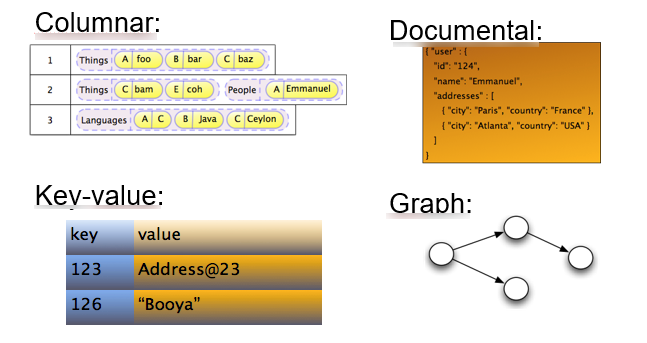
\includegraphics[width=0.6\textwidth]{nosql.png}
    \caption{Ejemplo de representación visual de modelos NoSQL}
    \label{fig:NoSQL}\cite{awsnosql}

\end{figure}
\vspace{0.5cm}
\printbibliography
\end{document}
